
\documentclass[11pt,a4paper]{article}
\usepackage{amsmath,amssymb,physics}
\usepackage{tikz}
\usetikzlibrary{arrows.meta,positioning,patterns,decorations.pathmorphing,calc}
\usepackage{tcolorbox}
\usepackage{tabularx}
\usepackage{microtype}
\usepackage{caption}
\captionsetup{justification=raggedright,singlelinecheck=false}
\usepackage{hyperref}

\title{From Keldysh to L\'evy: Unified EM Noise Framework for Trapped Ions}
\author{Ulrich Warring et al.}
\date{\today}

\begin{document}
\maketitle

\begin{abstract}
We derive a unified first-principles description of motional heating in trapped ions by integrating out electromagnetic degrees of freedom in the Keldysh formalism. 
All noise mechanisms---technical field fluctuations and collisional impulses---enter through stochastic current sources coupled via the trap's Green tensor. 
The resulting open-system dynamics take the form of a L\'evy--Khintchine generator (Gaussian diffusion + compound-Poisson jumps), with explicit links to scattering cross-sections. 
We provide experimentally discriminating observables, scattering-model formulas, and a practical inference protocol for reconstructing the jump-size L\'evy measure from stroboscopic measurements.
\end{abstract}

\tableofcontents


\section{Introduction}
Trapped ions are among the most sensitive probes of weak electromagnetic fields. 
Understanding and controlling their motional heating has been central since the earliest quantum logic and precision spectroscopy experiments \cite{Turchette2000,Wineland1998}. 
Traditionally, heating is modeled through spectral densities of electric field fluctuations $S_E(\omega)$, inferred by relating the ion's motional excitation rate to the environmental noise spectrum. 
This framework has successfully explained technical noise sources, Johnson noise in electrodes, and surface-potential fluctuations \cite{Brownnutt2015}. However, a complementary mechanism arises from discrete collision events: background gas flybys or scattering particles that impart sudden momentum kicks. 
These cannot be captured by Gaussian noise models alone. 
Instead, they produce intermittent heating signatures that are invisible to $S_E(\omega)$ alone.

We present here a unifying framework where both continuous noise and discrete collisions are subsumed into the language of stochastic currents $\mathbf{J}(\mathbf{r},t)$ mediated to the ion through the electromagnetic Green tensor $\mathbf{G}(\mathbf{r}_0,\mathbf{r};\omega)$. 
As illustrated schematically in Fig.~\ref{fig:em_mediation}, all differences reduce to the statistical character of the source currents: dense Gaussian baths vs.~sparse Poisson impulses.
%
\begin{figure}[t]
\centering
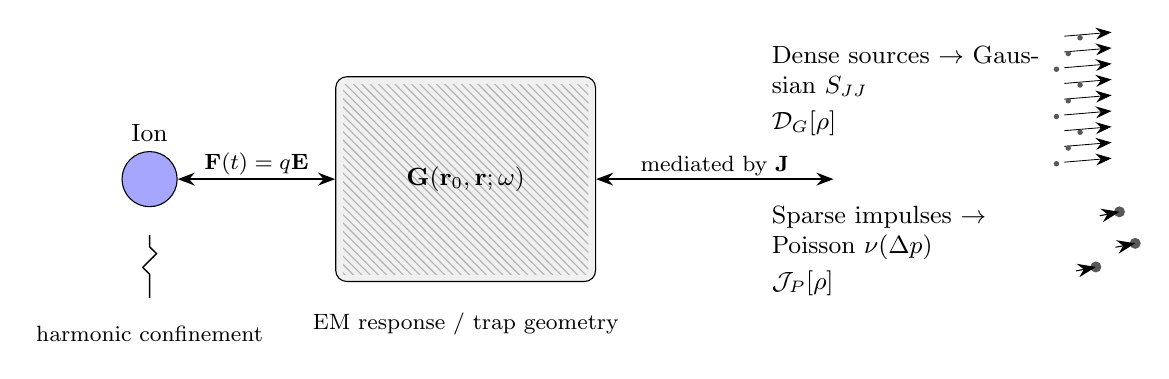
\begin{tikzpicture}[x=1cm,y=1cm,>=Stealth, node distance=2.cm]
  \small
  \tikzset{
    ion/.style={circle, minimum size=7mm, inner sep=0pt, draw=black, fill=blue!35},
    block/.style={draw, rounded corners, fill=gray!12, inner sep=6pt},
    annot/.style={align=left, text width=3.4cm},
    mathnote/.style={font=\footnotesize, inner sep=1pt}
  }
  \node[ion,label=above:{Ion}] (ion) {};
  \draw[line width=0.5pt] ([yshift=-0.35cm]ion.south) -- ++(0,-0.15)
    decorate[decoration=zigzag]{ -- ++(0,-0.5) } -- ++(0,-0.15);
  \node[below=1.4cm of ion, font=\footnotesize] {harmonic confinement};
  \node[block, minimum width=3.3cm, minimum height=2.6cm, right=of ion] (G) {};
  \begin{scope}
    \clip (G.south west) rectangle (G.north east);
    \fill[pattern=north west lines, pattern color=gray!60] 
      ($(G.south west)+(0.1,0.1)$) rectangle ($(G.north east)+(-0.1,-0.1)$);
  \end{scope}
  \node at (G) {$\mathbf{G}(\mathbf{r}_0,\mathbf{r};\omega)$};
  \node[mathnote, below=0.35cm of G] {EM response / trap geometry};
  \node[right=of G] (src) {};
  \node[annot, above=1.0 cm of src, anchor=west] (denseLab) {Dense sources $\rightarrow$ Gaussian $S_{JJ}$\\[2pt] $\mathcal{D}_G[\rho]$};
  \foreach \i in {0,...,8}{
    \draw[-{Stealth[length=2mm]}, line width=0.3pt]
      ($(denseLab.east)+(0.2,{-0.9+0.2*\i})$) -- ++(0.6,0.05);
    \fill[black!65] ($(denseLab.east)+({0.1+0.15*mod(\i,3)},{-0.92+0.2*\i})$) circle (0.035);
  }
  \node[annot, below=0.8cm of src, anchor=west] (sparseLab) {Sparse impulses $\rightarrow$ Poisson $\nu(\Delta p)$\\[2pt] $\mathcal{J}_P[\rho]$};
  \foreach \p/\dx in {0.5/0.9, -0.2/0.6, 0.1/1.1}{
    \fill[black!65] ($(sparseLab.east)+(\dx,\p)$) circle (0.07);
    \draw[-{Stealth[length=2.3mm]}] ($(sparseLab.east)+(\dx-0.25,\p-0.05)$) -- ++(0.25,0.05);
  }
  \draw[<->, line width=0.7pt] (ion) -- node[above, mathnote] {$\mathbf{F}(t)=q\mathbf{E}$} (G.west);
  \draw[<->, line width=0.7pt] (G.east) -- node[above, mathnote] {mediated by $\mathbf{J}$} ($(src)+(0.9,0)$);
  %\node[font=\footnotesize, align=center, below=1.0cm of G] 
   % %Unified picture: All mechanisms enter through EM coupling;\\ statistics of $\mathbf{J}(\mathbf{r},t)$ determine Gaussian vs.\ jump dynamics.};
\end{tikzpicture}
\caption{%
\textbf{Unified EM-mediated noise framework.}
All heating mechanisms—technical field noise and collisional impulses—couple to the trapped ion through the electromagnetic Green tensor $\mathbf{G}(\mathbf{r}_0,\mathbf{r};\omega)$ acting on stochastic current sources $\mathbf{J}(\mathbf{r},t)$. 
The distinction between Gaussian diffusion ($\mathcal{D}_G$) and compound-Poisson jumps ($\mathcal{J}_P$) arises from the statistical character of $\mathbf{J}$: dense sources yield Gaussian $S_{JJ}$, while sparse fly-by events produce a L\'evy measure $\nu(\Delta p)$ over momentum kicks.}
\label{fig:em_mediation}
\end{figure}
%
The theoretical development shows how integrating out the EM environment within the Keldysh formalism naturally yields a L\'evy--Khintchine form of the ion's master equation\,\cite{Sornette2006}: Gaussian diffusion plus compound-Poisson jumps. 
The experimental consequences are developed and we outline discriminants that separate Gaussian from non-Gaussian heating, introduce explicit scattering models, and provide inference protocols.
We also identify when the point-impulse approximation breaks down: for fast scatterers with trajectory extent comparable to the trap dimension, the spatial structure of $\mathbf{G}(\mathbf{r})$ induces directional and anisotropic heating. 

\section{Theoretical Framework: From Keldysh to L\'evy}

\subsection{System--Bath Setup}
We model a single trapped ion of charge $q$ and mass $m$, confined harmonically at frequency $\omega_t$ along $x$. 
The ion couples to the fluctuating electric field $\mathbf{E}(\mathbf{r}_0,t)$ at its equilibrium position $\mathbf{r}_0$, generated by stochastic currents $\mathbf{J}(\mathbf{r},t)$ in the environment. 
The Hamiltonian is
\begin{equation}
H = \frac{p^2}{2m} + \tfrac{1}{2} m \omega_t^2 x^2 - q x E_x(\mathbf{r}_0,t).
\end{equation}
The field obeys Maxwell's equations with sources $\mathbf{J}$, and the ion couples linearly via $H_{\text{int}} = -q x E_x$.

\subsection{Electromagnetic Green Tensor}
The electric field is expressed through the dyadic Green tensor $\mathbf{G}$ relating currents to fields in frequency space,
\begin{equation}
\mathbf{E}(\mathbf{r}_0,\omega) = \mathrm{i}\mu_0 \omega \int d^3r\, \mathbf{G}(\mathbf{r}_0,\mathbf{r};\omega) \mathbf{J}(\mathbf{r},\omega).
\end{equation}
Here $\mathbf{G}$ satisfies the Helmholtz equation 
\begin{equation}
\left[\nabla\times\nabla\times - \frac{\omega^2}{c^2}\varepsilon(\mathbf{r},\omega)\right]\mathbf{G}(\mathbf{r},\mathbf{r}';\omega) = \delta(\mathbf{r}-\mathbf{r}')\mathbf{I}.
\end{equation}
The permittivity $\varepsilon(\mathbf{r},\omega)$ encodes electrode/dielectric response; in practice $\mathbf{G}$ is computed numerically for trap geometry.

\subsection{Keldysh Formalism}
The ion+EM+bath system is described by a Keldysh action \cite{Kamenev2011}, doubling fields on forward/backward contours. 
Integrating out EM modes yields an effective action for the ion with force-force correlator
\begin{equation}
S_F(\omega) = q^2 \int d^3r d^3r'\, G_{x\alpha}(\mathbf{r}_0,\mathbf{r};\omega)\, S_{JJ}^{\alpha\beta}(\mathbf{r},\mathbf{r}';\omega)\, G^*_{x\beta}(\mathbf{r}_0,\mathbf{r}';\omega).
\label{eq:SF}
\end{equation}
\textit{Key result:} all environmental noise enters via $S_F(\omega)$, the current spectrum $S_{JJ}$ filtered by trap response $|\mathbf{G}(\omega)|^2$.

\subsection{Gaussian Bath $\to$ Diffusion}
For dense, weakly coupled baths, $\mathbf{J}$ is Gaussian with correlations $S_{JJ}$. 
The effective master equation is of Lindblad form
\begin{equation}
\dot{\rho} = -\mathrm{i}[H_0,\rho] + \Gamma_\uparrow \mathcal{D}[a^\dagger]\rho + \Gamma_\downarrow \mathcal{D}[a]\rho,
\end{equation}
with rates $\Gamma_{\uparrow,\downarrow} \propto S_F(\pm\omega_t)$. 
The heating rate is
\begin{equation}
\Gamma_{\text{heat}} = \Gamma_\uparrow - \Gamma_\downarrow = \frac{x_0^2}{\hbar^2}\left[S_F(+\omega_t) - S_F(-\omega_t)\right],
\end{equation}
with $x_0=\sqrt{\hbar/(2m\omega_t)}$. 
In equilibrium, detailed balance gives $S_F(-\omega_t)/S_F(+\omega_t)=e^{-\hbar\omega_t/k_BT}$.

\subsection{Poisson Bath $\to$ Jumps}
For sparse scatterers, $\mathbf{J}$ is a sum of impulses $\mathbf{j}_k(t-t_k)$. 
The effective dynamics are compound-Poisson: each event imparts momentum $\Delta p$, with rate $\lambda$ and distribution $\nu(\Delta p)$. 
The generator is
\begin{equation}
\mathcal{J}_P\rho = \lambda \int d(\Delta p)\, \nu(\Delta p)\,\left[e^{-\mathrm{i}\Delta p x/\hbar}\rho e^{+\mathrm{i}\Delta p x/\hbar}-\rho\right].
\end{equation}

\subsection{Unified L\'evy--Khintchine Form}
The full ion master equation is thus
\begin{equation}
\dot{\rho} = -\mathrm{i}[H_0,\rho] + \mathcal{D}_G[\rho] + \mathcal{J}_P[\rho],
\label{eq:levy-box}
\end{equation}
a L\'evy--Khintchine generator: Gaussian diffusion $\mathcal{D}_G$ plus compound-Poisson jumps $\mathcal{J}_P$.

\paragraph{Crossover regimes and dominance criteria.}
The relative importance of diffusion versus jumps is set by dimensionless ratios:
\begin{equation}
\frac{\text{jump heating}}{\text{Gaussian heating}} 
\sim \frac{\lambda \langle (\Delta p)^2 \rangle}{x_0^2 S_F(\omega_t)/\hbar^2},
\quad
\frac{\text{events per measurement}}{\text{one}} 
\sim \lambda \tau.
\end{equation}
Three regimes emerge naturally:
\begin{itemize}
\item \textbf{Diffusive limit} ($\lambda \tau \gg 1$, small $\langle(\Delta p)^2\rangle$): 
  Jumps coalesce into effective Gaussian noise; 
  $\kappa_3, \kappa_4 \to 0$; 
  Allan variance $\sigma_A^2(\tau) \propto \tau^{-1}$.
\item \textbf{Intermediate regime} ($\lambda \tau \sim 1{-}10$): 
  Both terms in Eq.~\eqref{eq:levy-box} contribute comparably; 
  non-Gaussian cumulants measurable ($\kappa_3/\kappa_2^{3/2} \sim 0.3{-}1$); 
  Allan variance shows rollover near $\tau \sim 1/\lambda$ 
  (Table~1, Sec.~3).
\item \textbf{Poisson limit} ($\lambda \tau \ll 1$, large $\langle(\Delta p)^2\rangle$): 
  Discrete, resolvable jumps dominate; 
  waiting-time statistics exponential; 
  $P(\Delta n)$ determined by $\nu(\Delta n)$ directly.
\end{itemize}
Experimentally, the intermediate regime is often the most informative: 
it separates mechanisms via higher-order statistics while still accumulating 
measurable events on laboratory timescales.
Table~1 (Sec.~3) provides experimentally accessible discriminants 
optimized for this intermediate regime, where neither limit dominates 
and model selection becomes nontrivial.

\subsection{Multiple microscopic sources within each regime}
While the L\'evy--Khintchine form (Eq.~\ref{eq:levy-box}) distinguishes 
Gaussian diffusion, compound-Poisson jumps, and heavy-tailed processes as 
\emph{statistical regimes}, each regime can in practice host several 
microscopic contributions. In the Gaussian sector, Johnson noise, surface 
patch fluctuations, and technical pickup all superpose in the current 
spectrum $S_{JJ}$, yielding an effective diffusion rate. In the Poisson 
sector, background gas collisions, cosmic ray events, and photoelectron 
kicks all contribute additively to the jump measure 
$\nu(\Delta p) = \sum_i \nu_i(\Delta p)$. 
Even in the heavy-tailed case, if multiple scattering mechanisms are present, 
the \emph{heaviest tail dominates} the asymptotic behavior: the effective 
tail exponent $\alpha$ is set by whichever process has the smallest $\alpha$ 
(slowest decay). Thus, a single long-range Coulomb scatterer can mask 
Langevin collisions at large $\Delta p$.

\paragraph{When mechanisms can be separated.}
While statistical discriminants measure the aggregate within each regime, 
independent variation of physical parameters can isolate contributions:
\begin{itemize}
\item \textbf{Controlled pressure scans} separate gas collisions $(\lambda \propto n_g)$ from fixed backgrounds (cosmic rays, technical noise).
\item \textbf{Temporal modulation} separates temperature-dependent 
  resonances (e.g., charge exchange with seasonal/diurnal T variation) 
  from constant sources.
\item \textbf{Trap orientation relative to Earth} can reveal cosmic ray 
  directionality vs. isotropic local sources.
\end{itemize}
In contrast, decomposing \emph{within} a sector (e.g., separating Johnson 
noise from patch-potential fluctuations in the Gaussian $S_{JJ}$) typically 
requires material-specific modeling or dedicated electrode studies 
\cite{Brownnutt2015}.

The inference protocol (Sec.~5) accounts for this by fitting 
\emph{mixture models}: a dominant Gaussian background plus 
one or more Poisson processes, with relative weights 
determined from data rather than assumed a priori.

\subsection{From Momentum to Phonon Jumps}
Experimentally, jumps are resolved in motional phonon number $n$. 
Momentum transfer $\Delta p$ maps to phonon transitions via
\begin{equation}
\nu(\Delta n) = \int d(\Delta p)\,\nu(\Delta p)\,\sum_{n'} P_{n\to n'}(\Delta p)\, \delta(\Delta n-(n'-n)),
\end{equation}
with $P_{n\to n'}(\Delta p)=|\langle n'|e^{-\mathrm{i}\Delta p x/\hbar}|n\rangle|^2$. 
This connects scattering cross-sections $d\sigma/d\Omega$ to measurable $\nu(\Delta n)$ (see Sec.~6).

\paragraph{Takeaway.} 
The ion's heating is universally described by Eq.~\eqref{eq:levy-box}, independent of microscopic mechanism. 
The experimentally accessible regime is often \emph{intermediate}, where $\lambda \tau \sim 1{-}10$ and both Gaussian and jump terms contribute measurably. 
Section~3 develops observables—cumulants, waiting times, Allan variance—that discriminate $\mathcal{D}_G$ versus $\mathcal{J}_P$ even when both are present simultaneously.


\begin{table}[h]
\centering
\renewcommand{\arraystretch}{1.2}
\begin{tabularx}{\textwidth}{>{\raggedright\arraybackslash}p{3.2cm}
                                  >{\raggedright\arraybackslash}X
                                  >{\raggedright\arraybackslash}X
                                  >{\raggedright\arraybackslash}X
                                  >{\raggedright\arraybackslash}p{2.8cm}}
\hline
\textbf{Observable} 
& \textbf{Gaussian bath} 
& \textbf{Compound-Poisson} 
& \textbf{Heavy-tailed L\'evy} 
& \textbf{Typical exp. access} \\
\hline
Skewness $\kappa_3/\kappa_2^{3/2}$ 
& $\to 0$ 
& $\sim 0.3{-}1$ 
& $\gg 1$, diverges with $\tau$ 
& $\sim 10^4$ shots \\

Waiting-time PDF 
& No distinct scale 
& Exponential (Poisson) 
& Power-law or stretched 
& $\sim 10^3$ events \\

Allan variance $\sigma_A^2(\tau)$ slope 
& $\propto \tau^{-1}$ (diffusive) 
& Rollover near $\tau \sim 1/\lambda$ 
& Anomalous slope $\neq -1$ 
& hours of trace \\

Jump-size distribution $P(\Delta n)$ 
& Gaussian tails 
& Exponential cutoff 
& Power-law $\propto \Delta n^{-\alpha-1}$ 
& $\sim 10^5$ shots \\

Sideband asymmetry vs.\ $\omega$ 
& Structured ($1/f$, lines) 
& Flat up to $1/\tau_{\rm coll}$ 
& Similar to Poisson (broadband) 
& $\sim 10^2$ scans \\
\hline
\end{tabularx}
\caption{Experimentally distinguishable signatures across three classes of noise: Gaussian field noise, compound-Poisson collisions, and heavy-tailed L\'evy processes. \emph{Note:} Real traps often exhibit mixed mechanisms; relative weights can be inferred by fitting linear combinations of the above signatures.}
\end{table}
% Table placeholder (content already provided earlier)
\section{Observable Signatures and Scattering Models}
The unified L\'evy--Khintchine generator (Eq.~\ref{eq:levy-box}, Sec.~2.6) predicts 
that ion heating arises from a combination of Gaussian diffusion and compound-Poisson jumps. 
We now develop experimentally distinguishable signatures that allow independent extraction of these components.

\noindent\textbf{(a) Langevin induced-dipole scattering}\quad
\emph{Regime:} Low-energy ion--neutral collisions with polarizable neutral ($E \lesssim 1$~eV).\\
\emph{Cross-section:}
\[
\frac{d\sigma}{d\Omega} = 
\frac{\alpha e^2}{8\pi\epsilon_0^2 \mu^2 v^4}\,
\frac{\sin^2\theta}{(1-\cos\theta)^4},
\]
with $\alpha$ the neutral polarizability. The total Langevin cross-section is 
$\sigma_{\rm L} = \pi e\sqrt{\alpha/(\epsilon_0 E)} \propto E^{-1/2}$.\\
\emph{Key feature:} Soft divergence at small $\Delta p$ (forward scattering), cut off by quantum diffraction $b_{\min}\sim \hbar/\mu v$.\\
\emph{Consequence:} $\nu(\Delta p)$ has enhanced small-$\Delta p$ weight; CLT $\to$ near-Gaussian heating but with fat tails.\\
\emph{Relevant systems:} Ca$^+$/Sr$^+$/Ba$^+$ with H$_2$, N$_2$, Ar backgrounds.

\textit{Universal behavior:} 
The Langevin form is \emph{universal} in the sense that it depends only on the neutral's polarizability $\alpha$, not on molecular details. 
This implies that $\nu(\Delta p)$ is parametrized by just $\alpha$ and the velocity distribution $f(v)$, reducing the inference problem to fitting $\lambda$ (or equivalently $n_g$) and $T$ from experimental data.
Departures from universality—resonant charge exchange, short-range chemistry, or high-energy collisions—introduce additional structure in $\nu(\Delta p)$ and require species-specific cross-sections.

\medskip
\noindent\textbf{(b) Hard-sphere scattering}\quad
\emph{Regime:} Classical collisions with effective radius $R$.\\
\emph{Cross-section:}
\[
\frac{d\sigma}{d\Omega} = \frac{R^2}{4\pi}.
\]
\emph{Key feature:} Isotropic scattering, momentum transfer peaked at $|\Delta p|=2\mu v$.\\
\emph{Consequence:} $\nu(\Delta p)$ becomes sharply peaked, yielding bimodal $P(\Delta n)$.\\
\emph{Relevant systems:} Test gases (He, Ne) in controlled background studies.

\medskip
\noindent\textbf{(c) Resonant charge-exchange}\quad
\emph{Regime:} Ion--atom collisions with same species (e.g.\ Ca$^+$ + Ca).\\
\emph{Cross-section:}
\[
\sigma(v) \approx \frac{\pi a_0^2}{1+(v/v_0)^2},
\]
with $v_0\sim \sqrt{\Delta E/\mu}$ from state energy defect $\Delta E$.\\
\emph{Key feature:} Strong velocity dependence; event rate $\lambda\propto n_g\langle v\sigma(v)\rangle$ inherits thermal modulation.\\
\emph{Consequence:} Waiting-time distribution becomes $T$-dependent; seasonal/diurnal modulations possible.\\
\emph{Relevant systems:} Ca$^+$, Yb$^+$ with neutral Ca, Yb vapor.

\medskip
\noindent\textbf{(d) Coulomb scattering (stray charges)}\quad
\emph{Regime:} Fly-by electrons/ions at distance $b\gg L_{\rm trap}$.\\
\emph{Cross-section:} Rutherford form,
\[
\frac{d\sigma}{d\Omega} \propto \frac{1}{\sin^4(\theta/2)}.
\]
\emph{Key feature:} Extremely long range; strong small-angle divergence.\\
\emph{Consequence:} Dominates if stray charges or cosmic rays penetrate; leads to anisotropic heating.\\
\emph{Relevant systems:} Cosmic ray backgrounds, photoionization byproducts.

\section{Spatial Coherence Effects}

\begin{tcolorbox}[title=Fast scatterers: spatial coherence effects]
For a moving scatterer with trajectory 
$\mathbf{r}_k(t)=\mathbf{r}_0+\mathbf{v}t$, 
the current density is
\[
\mathbf{j}_k(\mathbf{r},t) = \mathbf{j}^{(0)}_k(t)\,
\delta^{(3)}(\mathbf{r}-\mathbf{r}_k(t)).
\]
The force spectrum becomes
\[
F_k(\omega) = q \int dt\, e^{i\omega t}\,
\mathbf{G}(\mathbf{r}_0,\mathbf{r}_k(t);\omega)\cdot
\mathbf{j}^{(0)}_k(t).
\]

\textbf{Velocity regimes:}
\begin{itemize}\itemsep0.2em
\item Thermal background ($v \sim 500$~m/s, $\tau_{\rm coll}\sim 10$~ps): 
$v\tau_{\rm coll}\sim 5$~nm $\ll L_{\rm trap}$ $\to$ point-impulse limit.
\item Fast cosmics ($v\sim 0.1c$, $\tau_{\rm coll}\sim 1$~ps): 
$v\tau_{\rm coll}\sim 30~\mu$m $\sim L_{\rm trap}$ $\to$ extended-coherence regime.
\end{itemize}

\textbf{Impact:} Spatial variation of $\mathbf{G}$ introduces directional coupling, 
$|F_k(\omega)|^2 \propto |\hat{\mathbf{v}}\cdot\nabla\mathbf{G}|^2$, 
breaking isotropy. 

\textbf{Observable:} Anisotropic heating as a function of trap orientation relative to a collimated beam or fast flux (see Fig.~\ref{fig:trajectory_coherence}).
\end{tcolorbox}
\begin{figure}[h]
\centering
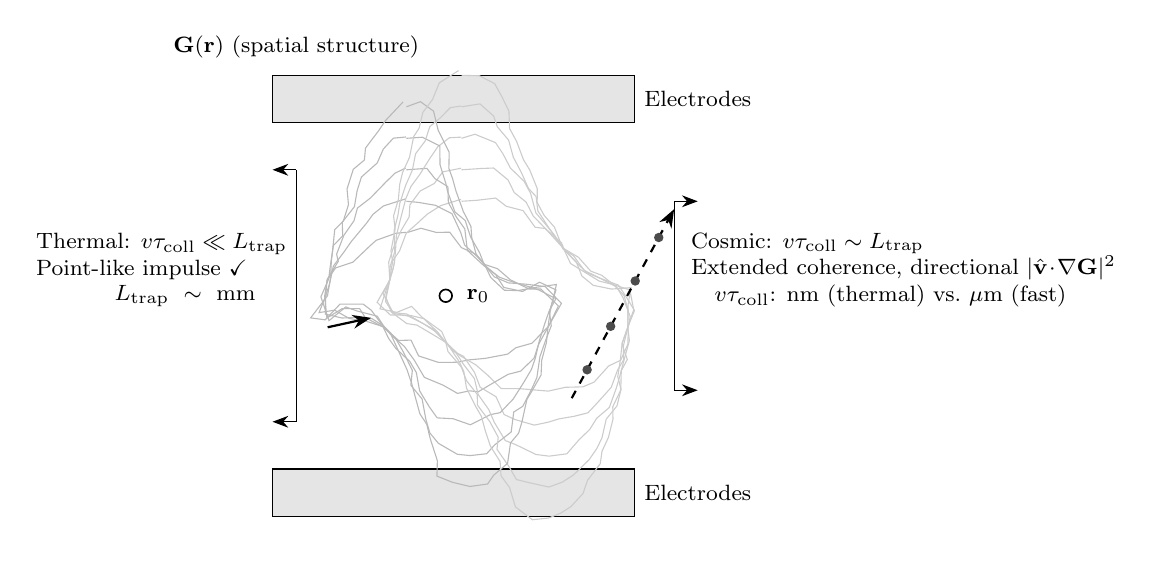
\begin{tikzpicture}[x=1cm,y=1cm,>=Stealth]
  \small
  \def\W{4.6}
  \def\H{6.2}
  \def\gap{3.2}
  \node at (0,0) {};
  \draw[fill=gray!20] (-1.5,  \gap/2+0.6) rectangle (\W-1.5,  \gap/2+1.2);
  \draw[fill=gray!20] (-1.5, -\gap/2-1.2) rectangle (\W-1.5, -\gap/2-0.6);
  \node[font=\footnotesize] at (\W-1.5+0.8,  \gap/2+0.9) {Electrodes};
  \node[font=\footnotesize] at (\W-1.5+0.8, -\gap/2-0.9) {Electrodes};
  \begin{scope}
    \clip (-1.5, -\H/2) rectangle (\W-1.5, \H/2);
    \foreach \a in {0.8,1.2,1.6,2.0,2.4}{
      \draw[gray!55, decorate, decoration={random steps, segment length=2mm, amplitude=0.6mm}]
        plot[smooth cycle, tension=1] coordinates{
          (-0.8,0) (0.2,\a) (1.2,0.4) (2.0,-0.2) (1.0,-\a) (-0.1,-0.4)};
      \draw[gray!40, decorate, decoration={random steps, segment length=2mm, amplitude=0.5mm}]
        plot[smooth cycle, tension=1] coordinates{
          (0.0,0.2) (0.9,\a+0.4) (2.2,0.6) (3.0,-0.4) (2.0,-\a-0.4) (0.7,-0.6)};
    }
  \end{scope}
  \node[font=\footnotesize, anchor=south] at (-1.2, \H/2-0.2) {$\mathbf{G}(\mathbf{r})$ (spatial structure)};
  \filldraw[fill=white, draw=black, line width=0.6pt] (0.7,0) circle (0.08);
  \node[font=\footnotesize, anchor=west] at (0.85,0) {$\mathbf{r}_0$};
  \draw[thick, -Stealth] (-0.8, -0.4) -- ++(0.55,0.12);
  \node[font=\footnotesize, align=left, anchor=east] at (-1.2,0.5)
    {Thermal: $v\tau_{\rm coll} \ll L_{\rm trap}$\\Point-like impulse \checkmark};
  \draw[thick, dashed, -Stealth] (2.3, -1.3) -- (3.6, 1.1);
  \foreach \t in {0.15,0.38,0.62,0.85}{
    \fill[black!70] ($(2.3, -1.3)!{\t}!(3.6,1.1)$) circle (0.06);
  }
  \node[font=\footnotesize, align=left, anchor=west] at (3.7, 0.5)
    {Cosmic: $v\tau_{\rm coll} \sim L_{\rm trap}$\\Extended coherence, directional $|\hat{\mathbf{v}}\!\cdot\!\nabla\mathbf{G}|^2$};
  \draw[very thin] (-1.2,-\gap/2) -- (-1.2,\gap/2);
  \draw[-{Stealth[length=2mm]}] (-1.2,\gap/2) -- ++(-0.3,0);
  \draw[-{Stealth[length=2mm]}] (-1.2,-\gap/2) -- ++(-0.3,0);
  \node[font=\footnotesize, align=center, anchor=east] at (-1.6,0) {$L_{\rm trap}\ \sim\ \mathrm{mm}$};
  \draw[very thin] (\W-1.0,-1.2) -- (\W-1.0,1.2);
  \draw[-{Stealth[length=2mm]}] (\W-1.0,1.2) -- ++(0.3,0);
  \draw[-{Stealth[length=2mm]}] (\W-1.0,-1.2) -- ++(0.3,0);
  \node[font=\footnotesize, align=center, anchor=west] at (\W-0.6,0)
    {$v\tau_{\rm coll}$: nm (thermal) vs.\ $\mu$m (fast)};
\end{tikzpicture}
\caption{%
\textbf{Spatial coherence effects for fast scatterers.}
When the trajectory extent $v\tau_{\rm coll}$ approaches the trap dimension $L_{\rm trap}$, $\mathbf{G}(\mathbf{r})$ varies along the path, leading to directional coupling $|F_k(\omega)|^2 \propto |\hat{\mathbf{v}}\!\cdot\!\nabla\mathbf{G}|^2$ and anisotropic heating.}
\label{fig:trajectory_coherence}
\end{figure}
\section{Inference Protocol}

\paragraph{Recommended stroboscopic sequence.}
\begin{enumerate}\itemsep0.2em
  \item Prepare motional ground state $\lvert n=0\rangle$ (or a calibrated thermal $\langle n\rangle$).
  \item Wait time $\tau$ (free evolution under noise).
  \item Read out $n$ via sideband thermometry or time-of-flight.
  \item Repeat $N$ times $\Rightarrow$ histogram $P(n\,|\,\tau)$ and time series $n(t)$.
\end{enumerate}

\paragraph{Sample-size guidelines.}
\begin{table}[h]
\centering
\renewcommand{\arraystretch}{1.15}
\begin{tabularx}{0.9\textwidth}{>{\raggedright\arraybackslash}X>{\raggedleft\arraybackslash}p{4.2cm}}
\hline
\textbf{Target quantity} & \textbf{Required shots/events (order-of-magnitude)} \\
\hline
Detect $\kappa_3 \neq 0$ at $3\sigma$ & $\sim 10^4$ stroboscopic shots \\
Reconstruct $\nu(\Delta n)$ (5 bins)  & $\sim 10^5$ shots \\
Test heavy-tail exponent $\alpha$      & $\sim 10^6$ events \\
Allan variance rollover near $1/\lambda$ & hours of continuous trace \\
Sideband asymmetry vs.\ $\omega$ map   & $\sim 10^2$ frequency scans \\
\hline
\end{tabularx}
\end{table}

\paragraph{Systematic error sources (and mitigations).}
\begin{itemize}\itemsep0.2em
  \item \textbf{Readout noise} smears $P(\Delta n)$: calibrate with known coherent kicks and deconvolve.
  \item \textbf{Motional dephasing} during $\tau$: ensure $\tau \ll 1/\Gamma_{\rm dephase}$ or include dephasing in the likelihood model.
  \item \textbf{Multi-ion coupling}: analyze in normal-mode basis; report mode-resolved $\nu(\Delta n)$.
  \item \textbf{Background drift / non-stationarity}: use sliding-window estimators for $\lambda(t)$, $\langle \Delta n \rangle(t)$.
\end{itemize}

\paragraph{Estimation outputs (minimum set).}
\begin{itemize}\itemsep0.2em
  \item Cumulants $\kappa_2(\tau)$, $\kappa_3(\tau)$, $\kappa_4(\tau)$; Gaussian vs.\ non-Gaussian decision.
  \item Change-point inference of jump times $\{t_k\}$ and sizes $\{\Delta n_k\}$; empirical $\hat{\nu}(\Delta n)$.
  \item Rollover in $\sigma_A^2(\tau)$ and sideband asymmetry vs.\ $\omega$ to constrain $|\mathbf{G}(\omega)|^2$.
\end{itemize}% Inference protocol placeholder

\bibliographystyle{unsrt}
\bibliography{refs}
\end{document}
